The neighborhood classes are all subclasses of the super class \class{Neighborhood} such that they can easily be 
combined with the search procedures. The methods of neighborhoods are illustrated in figure \ref{fig_neighborhood}. \\
\begin{figure}[!b]
\begin{center}
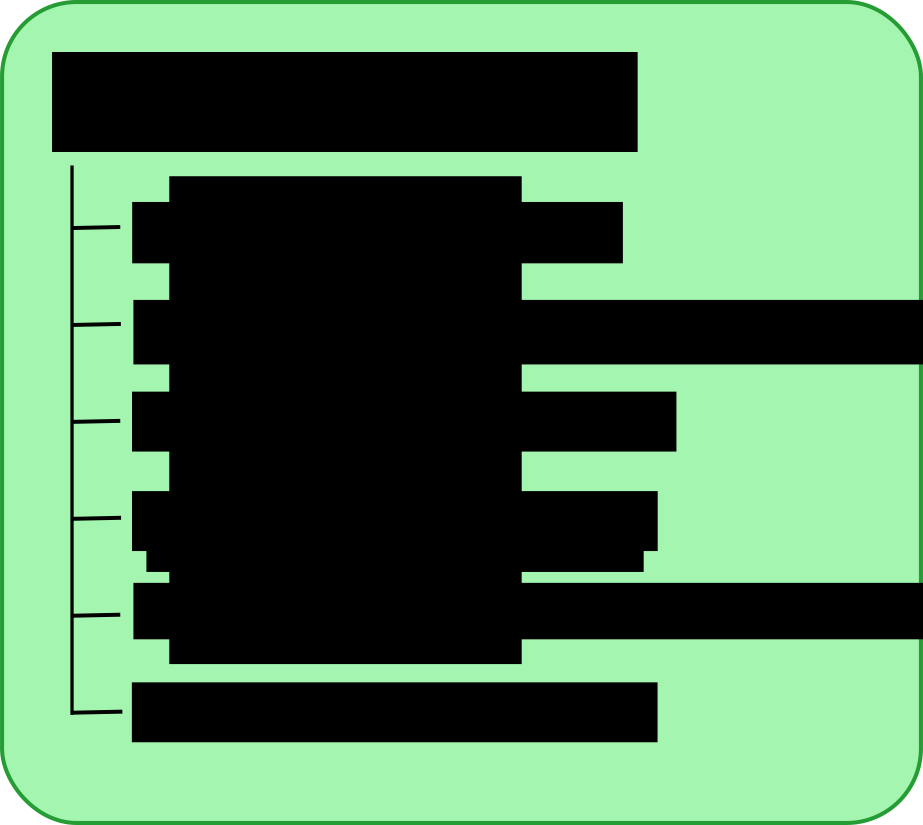
\includegraphics[width=0.9\linewidth]{neighborhood}\caption{The methods all Neighborhood classes needs to implement.} 
\label{fig_neighbborhood}
\end{center}
\end{figure}
All \class{Neighborhoods} implemented uses a step functions that changes value of a single independent variable, from 
0 to 1 or vise versa since all variables are binary. A neighborhood operation is stored in an a \class{Move} that 
contains a pointer to the variable used, the variables change in value, and the change to the quality vector $Q$, 
once computed. The change in the quality vector is referred to at the \emph{delta vector}. \\ 
The \class{Neighborhood} classes that are implemented are shown in table \ref{tab_neighb}. \\  
\begin{table}[!t]
\centering
\begin{tabular}{|l|l|}
\hline
class                          & Heuristic                                          \\ \hline
\class{FlipNeighborhood}     & All variables                                      \\ \hline
\class{RestrictedFlipNE}     & A Random subset of the variables	               \\ \hline
\class{ConflictOnlyNE}       & Variables in unsatisfied constraints           \\ \hline
\class{RandomConflictFlipNE} & Variables from a random unsatisfied constraint \\ \hline
\end{tabular}
\caption{Table of \class{Neighborhood} classes}
\label{tab_neighb}
\end{table}
The method \method{next()} creates new \class{Move} object and returns a pointer to it. If all the 
different neighborhood operation has been returned the method returns a pointer to \textbf{NULL} instead. To know when 
a neighborhood has been fully explored, counters and iterators are used depending on the neighborhood. These are 
reseted when returning \textbf{NULL} or the method \method{commitMove(move)} is called. The \class{Move} created only 
contain the variable and its suggested change in value, the delta vector is not computed yet. \\ 
Method \method{nextRandom()} gives a random neighborhood operation without changing the.  \\ 
Method \method{calculateDelta(move)} takes a \class{Move} pointer as argument and propagate the change through the 
dependency digraph using the propagation queue of the variable. The method identical for all the \class{Neighborhood} 
classes implemented. A neighborhood operation that calculate the delta change if variable $x_i$ would change value is 
describe with the following step:
\begin{enumerate} 
 \item Reset delta value of invariants in quality vector $Q$
 \item Send delta value of $x_i$ to neighbor invariant in DDG.
 \item For each invariant $inv$ in propagation queue of $x_i$, calculate $inv$s delta value, if it is not zero, send 
it to neighbor invariants in DDG. 
 \item If a variables delta value is not allowed, by a oneway constraint, reset all delta values of invariant in 
the propagation queue.
 \item Otherwise set $move$s delta quality vector. 
\item return if the $move$ is an allowed neighborhood operation. 
\end{enumerate}
The delta values of the invariants can be reset by calculating delta value, when no change is send. The reason for 
resetting them is only to make sure their queue of changes is empty before the next neighborhood operation. \\ 
To perform a step the method \method{commitMove(move)} is called with a pointer to the \class{Move} that used be used.  
\method{commitMove(move)} use the delta value calculated by \method{calculateDelta(move)} to update the value of 
invariants. The delta value needs to be recomputed since other neighborhood operation might have been suggested. Once 
the delta values of invariants have been computed they can be added to their current value. Invariants that represent 
violation of a single constraint are kept in a hash map of they are non zero. If they change value from non zero to zero 
or vise versa, that hash map needs to be updated. The hash map is used by the two neighborhoods \class{ConflictOnlyNE} 
and \class{RandomConflictFlipNE} that only can be used when the current solution is infeasible. \\
A default method \method{compareMoves(move1,move2)} compares the delta vector of two \class{Move} pointers and returns 
0 if they are the same, 1 if if move1 is best and 2 otherwise. \\ 
The size of the neighborhood and the restriction applied to it, if any. Method \method{getSize()} returns the size of 
the current neighborhood, for \class{ConflictOnlyNE} and \class{RandomConflictFlipNE} the neighborhood size can change 
after each step. \\ 




